\section{Caracterización de los graduados por sede}

La integración de las bases del Observatorio reúne a 174.685 graduados de la Universidad Santo Tomás repartidos en sus seis sedes. El análisis que sigue describe el tamaño relativo de cada una, su trayectoria temporal, los programas que definen su perfil y la composición de su oferta entre pregrado y posgrado, para cerrar con una síntesis comparativa que contrasta el volumen con la participación agregada.

\subsection{Tamaño y peso de cada sede}

La distribución de graduados está fuertemente concentrada en la Sede Principal de Bogotá, que reúne 104.468 personas, es decir, alrededor de seis de cada diez graduados de toda la Universidad. A considerable distancia aparece Bucaramanga con 37.370 graduados, seguida por Tunja con 14.859 y la VUAD con 11.098. Las seccionales de Villavicencio y Medellín, con 7.030 y 3.374 graduados respectivamente, completan el conjunto como las de menor tamaño.

El número de registros académicos supera siempre al de personas, porque un mismo graduado puede haber obtenido más de un título en la Universidad. Esa brecha es más amplia precisamente donde la oferta de posgrados es más densa: en Bogotá los 115.473 registros frente a 104.468 personas reflejan una proporción apreciable de graduados que regresaron para cursar una especialización o una maestría, y en Tunja los 17.925 registros frente a 14.859 personas apuntan en el mismo sentido. En las sedes más jóvenes o de menor tamaño la diferencia entre registros y personas se estrecha, señal de que la formación posgradual todavía no ha generado allí la misma circulación de egresados.

\begin{figure}[H]\centering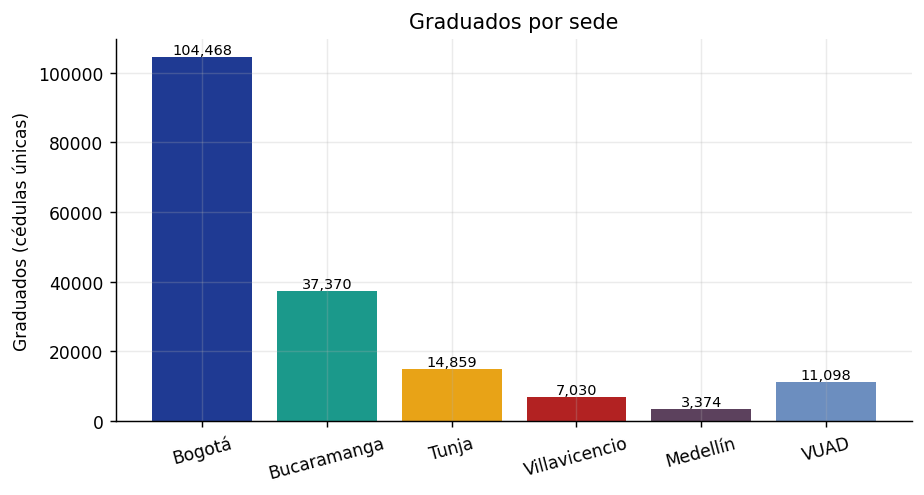
\includegraphics[width=0.82\linewidth]{figs_cruce/01_grad_seccional.png}\caption{Graduados por sede seccional. Bogotá concentra cerca del 60\% del total.}\label{fig:gradsec}\end{figure}

La Figura~\ref{fig:gradsec} hace visible el contraste de escalas: la Sede Principal no solo encabeza el conjunto, sino que multiplica varias veces el tamaño de cualquier seccional, lo que condiciona buena parte de las cifras agregadas que se presentan más adelante.

\subsection{Evolución histórica}

La cobertura temporal de la base se extiende entre 1970 y 2026. La Sede Principal de Bogotá aporta la serie más larga y voluminosa, con graduaciones que se remontan al inicio del periodo y un máximo histórico de 6.225 títulos en 1999, una cifra que ninguna otra sede se acerca a igualar. Las seccionales presentan trayectorias más recientes y picos de magnitud mucho menor: Bucaramanga alcanza su máximo en 2025 con 2.024 graduados, Tunja también en 2025 con 1.620, Villavicencio en 2024 con 921, la VUAD en 2018 con 902 y Medellín en 2023 con 238.

El arranque tardío de Villavicencio, cuyo pico se sitúa apenas en 2024, ilustra cómo varias seccionales se consolidaron como centros de graduación en fechas relativamente recientes, mientras Bogotá ya acumulaba décadas de egresados. El año 2026 se excluye de la lectura de tendencias por corresponder a un periodo todavía en curso, cuyos registros están incompletos.

\begin{figure}[H]\centering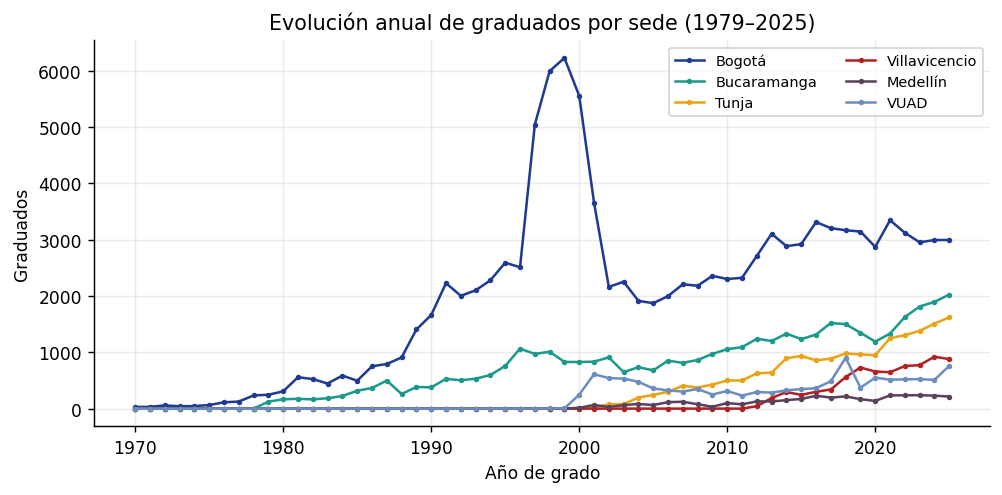
\includegraphics[width=0.82\linewidth]{figs_cruce/02_evolucion_seccional.png}\caption{Evolución anual de graduaciones por sede, 1970--2025.}\label{fig:evolucion}\end{figure}

La Figura~\ref{fig:evolucion} muestra estas trayectorias superpuestas y deja ver tanto el predominio sostenido de Bogotá como la incorporación escalonada de las demás sedes a lo largo de las últimas décadas.

\subsection{Programas dominantes}

El perfil formativo de la Universidad se define por un núcleo de programas de las ciencias jurídicas, económicas y administrativas. Derecho encabeza con holgura la lista, con 19.086 graduados, seguido por Contaduría Pública con 10.254. A continuación aparecen la Especialización en Derecho Administrativo con 8.887, Negocios Internacionales con 7.867 y Economía con 7.107, lo que confirma el peso de la formación posgradual jurídica dentro de la oferta.

Las ingenierías y la arquitectura ocupan un lugar destacado, con Ingeniería Civil (6.574) y Arquitectura (6.019) entre los diez programas más numerosos, acompañadas más abajo por Ingeniería Electrónica. La presencia de Administración de Empresas (6.085), Psicología (5.004) y Odontología (3.964) amplía el espectro hacia las ciencias sociales y de la salud. Las licenciaturas, vinculadas en buena medida a la educación a distancia, completan el cuadro con programas en educación preescolar, educación básica y filosofía y ciencias religiosas, que reflejan la vocación humanista y pedagógica de la institución.

\begin{figure}[H]\centering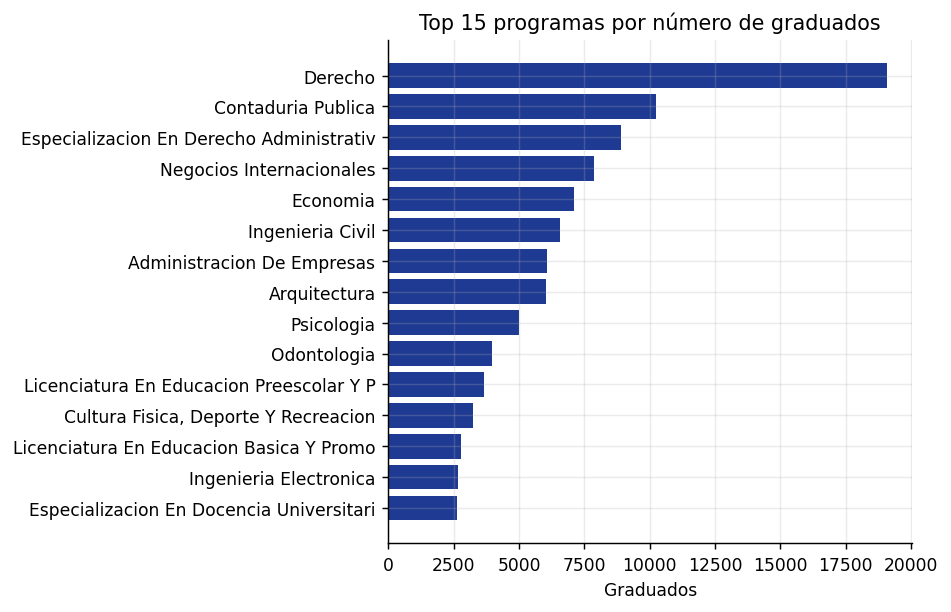
\includegraphics[width=0.82\linewidth]{figs_cruce/03_top_programas.png}\caption{Programas con mayor número de graduados en el conjunto de la Universidad.}\label{fig:topprog}\end{figure}

La Figura~\ref{fig:topprog} ordena estos programas según su volumen de graduados y permite apreciar el dominio de Derecho frente al resto de la oferta.

\subsection{Modalidad de formación}

La composición entre pregrado y posgrado, ahora disponible para las seis sedes, varía de manera notable. Bogotá combina 68.083 graduados de pregrado con 47.390 de posgrado, una proporción posgradual cercana al 41\% que da cuenta de una oferta madura de especializaciones y maestrías. Tunja presenta el perfil más orientado al posgrado, con 7.747 títulos posgraduales frente a 10.178 de pregrado, alrededor del 43\% del total. Bucaramanga, que ahora también reporta modalidad, suma 29.207 graduados de pregrado y 11.782 de posgrado, una proporción posgradual próxima al 29\%.

En el extremo opuesto, Villavicencio y la VUAD concentran su actividad en el pregrado: la primera reporta 5.893 graduados de pregrado frente a 1.726 de posgrado, y la VUAD, ligada a la educación a distancia, suma 9.129 títulos de pregrado por apenas 2.504 de posgrado, en ambos casos alrededor de un 22\% o 23\% posgradual. Medellín ocupa una posición intermedia, con 2.347 graduados de pregrado y 1.287 de posgrado, un peso del posgrado próximo al 35\%.

\begin{figure}[H]\centering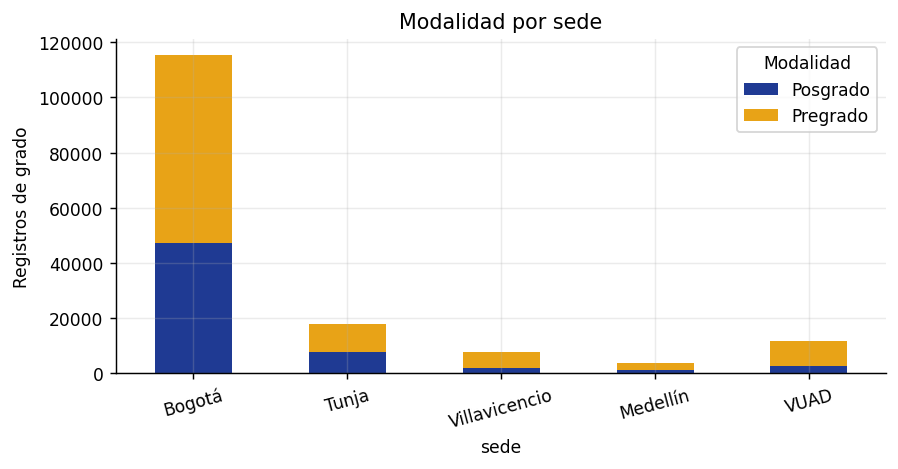
\includegraphics[width=0.82\linewidth]{figs_cruce/04_modalidad_seccional.png}\caption{Distribución de graduados entre pregrado y posgrado por sede.}\label{fig:modalidad}\end{figure}

La Figura~\ref{fig:modalidad} sintetiza estos contrastes y evidencia que la madurez posgradual está asociada a las sedes de mayor trayectoria, como Bogotá y Tunja.

\subsection{Síntesis comparativa por sede}

\begin{table}[H]\centering\scriptsize
\caption{Síntesis comparativa por sede: tamaño, formación y participación.}
\label{tab:seccional_sintesis}
\begin{tabular}{lrrrrrr}
\toprule
\rowcolor{ustaazul}\textbf{\color{white}Indicador} & \textbf{\color{white}Bogotá} & \textbf{\color{white}Bucaramanga} & \textbf{\color{white}Tunja} & \textbf{\color{white}Villavicencio} & \textbf{\color{white}Medellín} & \textbf{\color{white}VUAD} \\
\midrule
Graduados (personas) & 104.468 & 37.370 & 14.859 & 7.030 & 3.374 & 11.098 \\
Posgrado (\% títulos) & 41\% & 29\% & 43\% & 23\% & 35\% & 22\% \\
Programa principal & Derecho & Derecho & Derecho & Derecho & Arquitectura & Administracion D \\
Proveedor (SECOP) & 20,0\% & 28,2\% & 45,2\% & 38,0\% & 28,9\% & 19,9\% \\
Matriculado en RUES & 18,2\% & 29,0\% & 24,8\% & 24,2\% & 17,8\% & 23,3\% \\
Investigador (CvLAC) & 1,5\% & 1,3\% & 2,5\% & 1,2\% & 1,1\% & 0,6\% \\
Con $\geq$1 dimensión & 34,4\% & 49,1\% & 58,0\% & 52,2\% & 40,5\% & 36,4\% \\
\bottomrule
\end{tabular}
\\[2pt]{\scriptsize\color{ustagris} VUAD agrupa los centros de atención universitaria (educación a distancia).}
\end{table}

La tabla anterior reúne en un mismo cuadro el tamaño, la composición formativa y las tasas de participación de cada sede, y revela que el volumen de graduados no determina por sí solo la huella que dejan en el ámbito público, empresarial e investigativo. Tunja lidera la participación agregada: el 45,2\% de sus graduados figura como proveedor del Estado en SECOP y el 2,5\% aparece validado como investigador en CvLAC, las cifras más altas en ambas dimensiones, lo que la sitúa al frente en contratación pública e investigación pese a su tamaño intermedio. Bucaramanga destaca en el terreno de la matrícula mercantil, con un 29,0\% de sus graduados registrados en RUES, la proporción más alta de toda la Universidad. Bogotá, en cambio, presenta tasas comparativamente bajas, con un 20,0\% en SECOP y un 18,2\% en RUES, de modo que su enorme volumen de egresados convive con una intensidad de participación por persona menor que la de las seccionales más pequeñas.

\begin{cajahallazgo}
Cada sede dibuja un perfil propio que va más allá de su número de graduados. Las seccionales como Tunja, Villavicencio y Bucaramanga alcanzan tasas de inserción pública, empresarial e investigativa superiores a las de la Sede Principal, mientras Bogotá aporta el grueso del volumen pero con una huella por graduado más diluida. Estos perfiles diferenciados sirven de telón de fondo para el análisis de las dimensiones de participación que se desarrolla en las secciones siguientes.
\end{cajahallazgo}
